\chapter{Аналитический раздел}
\label{cha:analysis}

Выделение голосовой составляющей из аудио сигнала является частным случаем задачи разделения комбинации аудио сигналов на составляющие. Музыкальное произведение может быть записано как с использованием нескольких микрофонов, захватывающих разные источники, при этом изоляция источников будет ограничена, либо с использованием выделенной на каждый источник. Все записанные сигналы в последствии проходят процесс сведения для получения итоговой аудио записи. Тем самым конечный аудио сигнал можно представить в виде суммы отдельных источников с приминением фильтров к каждому источнику.

Математически это можно записать как:

\begin{equation}
 x(t) = \sum_{j=1}^{J} \sum_{\tau=-\infty}^{\infty} a_{j}(t-\tau, \tau)s_j(t-\tau)
\end{equation}

где 

\begin{itemize}
	\item $x$ -- итоговый аудио сигнал;
	\item $s_j$ -- сигнал источника;
	\item $J$ -- количество источников;
	\item $a_j$ -- фильтр, примененный к источнику в процессе сведения.
\end{itemize}

Если приминяемые фильтры являются линейными, то итоговый сигнал представляет собой линейную комбинацию. С другой стороны, к итоговому сигналу так же могут быть применены фильтры. С этой точки зрения сведенный сигнал перестает быть линейной суммой отдельных источников. 

Тем самым, итоговая запись, в контексте задачи выделения аудио источников, может быть определена по следующим категориям:

\begin{enumerate}
	\item Недостаточно или черезмерно определенные записи. Зависит от заранее известном числе источников. Например, запись с использованием нескольких микровонов считается черезмерно определенной, а запись с использованием одного микрофона считается недостаточно определенной.
	\item Мгновенные или свернутые записи. Зависит от информации о эффектах, примененных к итоговому сигналу.
	\item Записи, изменяющиеся или неизменающиеся во времени. Например запись, сделаная с использованием перемещающегося микрофона определяется как изменяющаяся во времени.
\end{enumerate}

Эта работа будет сфокусирована на обработке черезмерно определенной записью, предполагающеся мгновенной и неизменной во времени.

\section{Цифровое представление аудио сигналов}

Звук имеет три основных характеритичесих параметров: амплитуда, частота и фаза. Две последнии характеристики являются функциями времени, в то время как амплитуда определяет динамический диапозон. По этому в цифровом представлении аудио сигнала записываются изменения аплитуды как функция времени. Тем самым процесс отцифровки аналогового аудио сигнала является записью мгновенных амплитудных значений (дискретизация по амплитуда) в постоянные моменты времени (дискретизация по времени). Графическое представление дискретизации аналогового сигнала представлено на рисунке \ref{anal:atob}.

\begin{figure}
	\centering
	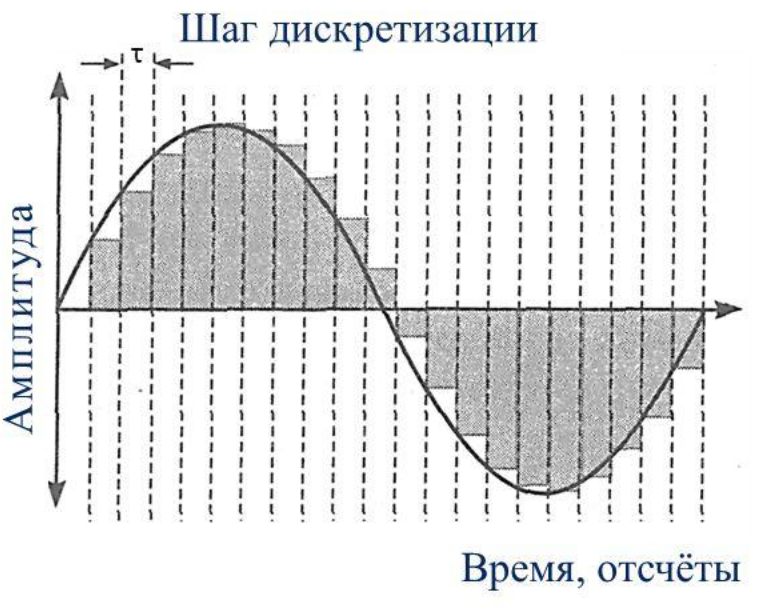
\includegraphics[width=\textwidth]{inc/img/analog-to-bin.png}
	\caption{Дискретизация аналогового сигнала}
	\label{anal:atob}
\end{figure}

Для определения периода записи амплитудных значений задается частота дискретизации. 

Существует теорема Котельникова\cite{Bikkenin}, утверждающая, что <<любую функцию $F(t)$, состоящую из частот от 0 до $f_1$, можно непрерывно передавать с любой точностью при помощи чисел, следующих друг за другом через $1/(2f_1)$ секунд>>.

При максимальной воспринимаемой человеческим ухом частоте в 20 кГц, по теореме Котельникова минимальная необходимая частота дискретизации должна быть 40 кГц.

Стандартная частота дискретизации аудио сигнала составляет 44,1 кГц, максимальная -- 192 кГц.

Для определения максимального значения амплитуды используется значение квантования (или разрядность), задающаяся в битах. В зависимости от используемого формата разрядность может быть 1, 8, 16, 24 и 32 бит.

Сравнение существующих форматов хранения цифрового аудио сигнала по квантованию и частоте дискретизации представлено в таблице \ref{anal:formats}.

\begin{table}
	\caption{\label{anal:formats}Сравнение цифровых аудиоформатов}
	\begin{center}
		\begin{tabular}{|p{0.4\textwidth}|p{0.3\textwidth}|p{0.3\textwidth}|}
			\hline
			Название формата & Квантование, бит & Частота дискретизации, кГц \\
			\hline
			WAVE (WAV) & 8; 16; 24; 32 & любая \\
			\hline
			AIFF & 8; 16; 24; 32 & 11,025; 22,05; 24; 32; 44,1; 48; 96; 192 \\
			\hline
			WavPack & 8; 16; 24; 32 & 6 -- 192 \\
			\hline
			FLAC & 4 -- 32 & до 192 \\
			\hline
			Lossless Predictive Audio Coder (LPAC) & 8; 16; 20; 24; & до 192 \\
			\hline
			LosslessAudio (LA) & 16 & 48 \\
			\hline
			Windows Media Audio 9 Lossless & 16; 24 & 8; 11.025; 16; 22.05; 32; 44.1; 48; 88.2; 96 \\
			\hline
			Apple Lossless (ALAC, ALE) & 16; 24 & 44.1; 48; 88.2; 96; 192 \\
			\hline
			MP3 & 16; 24 & до 48 \\
			\hline
		\end{tabular}
	\end{center}
\end{table}

\section{Существующие методы выделения источников}

\subsection{Метод главных компонент}
Метод главных компонент (англ. Principal Component Analysis) и анализ независимых компонент (англ. Independent Component Analysis) -- это статистические способы уменьшения размерности данных, который являлся объектом для исследований в области выделения аудио источников \cite{Lopez} \cite{Dadula}.

Основная идея этоих метода заключается в том, чтобы проецировать данные из временных рядов, таких как аудиозапись, в новые системы отсчета, которые основаны на некотором статистическом критерии. Эти оси являются статистически независимые в отличие от преобразования Фурье, где данные временной области проецируются на оси частот, которые могут перекрываться. Частотные оси в преобразовании Фурье остаются неизменными независимо от анализируемой части, тогда как в методе главных компонент и анализе независимых компонент оси являются динамическими и различны для каждой анализируемой части. После нахождения, оси, на которые происходит проецирование, могут быть разделены и инвертированы для нахождения источников, представленных в исходном сигнале.

В методе главных компонент мерой разделения осей является дисперсия. Оси рекурсивно выбираются в качестве направления, в которых дисперсия сигнала максимальна, что приводик к декорреляции во втором порядке между осями. Тем самым, основные компоненты амплитудной характеристики сигнала находятся на первых осях. Данный метод может быть использован как для сжатия информации, так и для выделения источников.

В анализе независимых компонент, четвертый момент, называющийся коэффициент эксцесса, используется в качестве критерия для нахождения новых систем отсчета. В теории вероятностей коэффициент эксцесса является мерой остроты пика распределения случайной величины или показателем <<негуссовости>> сигнала. Негативное значение коэффициента означает, что функция ресрпежедения вероятностей шире Гауссовского распределения, в то время как положительное значение -- уже. Тем самым в анализе независимых компонент сигнал разделяется на негауссовские независимые сигналы, а в методе главных компонент сигнал разделяется на гауссовские независимые сигналы.

Задача сводится к серии матричных произведений, представляющих свобой фильтры. В общем случае входной сигнал $X$ размерности $N$ из $M$ образцов (представляется матрицей размерности $NxM$) может быть приведен к сигналу $Y$ с использованием матрицы преобразования $W$ размерности $NxN$ как $Y^T = WX^T$. Такое преобразование проецирует сигнал на разные оси основываясь на матрице преобразования. Если размер полученного сигнала равен размер исходного сигнала, то преобразование называется ортогональным и оси перпендикулярны.

Эти операции называются преобразованиями без потерь из-за того, что исходный сигнал может быть восстановлен без потерь информации. Если один или несколько столбцов матрицы являются нулевыми, то такие операции называются преобразованиями с потерями и используются для фильтрации и сжатия данных. Преобразование считается биортогональным, когда исходная и результирующая оси перпендикулярны. Такое преобразование является без потерь. Метод главных компонент и анализ независимых компонент являются ортогональными и биортогональными соответственно.

Главной задачей яляеется получение матрицы преобразования.

\subsection{Факторизация неотрицательных матриц}

Факторизация неотризательных матриц (англ. Non-Negative Matrix Factorization) широко использовалась в области выделения источников в прошлом. Основная идея данного метода заключается в представлении матрицы $Y$ в виде комбинации базиса $B$ и активационного усиления $G$ как $Y=BG$. Базовый вектор предстовляет частотную характеристику источника в заданный момент времени, а вектор $G$ представляет усиление частот в любой момент времени. Таким временем $G$ является горизонтальным вектором вдоль времени.

В контексте задачи выделения аудио источников, если исходный сигнал является объединением двух источников, $S_1$ и $S_2$, так, что $Y = S_1 + S_2$, и базисные вектора двух источников вычисляются как $B_1$ и $B_2$, то исходный сигнал можно представить как $Y = B_1 G_1 + B_2 G_2$, где $G_1$ и $G_2$ -- соответсвующие активанционные усиления для двух источников, представленные в разные моменты времени. 

Для применения факторизации неотрицательных матриц необходимо, чтобы сигнал представлял из себя линейную комбинацию базисных векторов. Для $K$ источников:

\begin{equation}
X_{i,j} = \sum_{k=1}^{K} B_{i,k} G_{k, j}
\end{equation}

Расхождение между $X$ и $BG$ должно быть минимизировано, чтобы гарантировать, что найденные аудио источники представляют в комбинации исходный сигнал:

\begin{equation}
{B, G} = argmin_{B, G >= 0} D (X, BG)
\end{equation}

где $D$ является функцией расхождения, которая может быть:

\begin{enumerate}
	\item евклидовым расстоянием:
	\begin{equation}
	D (A, B) = ||A-B||^2 = \sum_{ij}(A_{ij} - B_{ij})^2
	\end{equation}
	\item дивергенцией Кулбека-Лейблера:
	\begin{equation}
		D (A, B) = \sum_{ij} (A_{ij} \log\frac{A_{ij}}{B_{ij}} - A_{ij} + B_{ij})
	\end{equation}
\end{enumerate}

Для этой дивергенции применяется алгоритм мультипликативного обновления \cite{DLee}:

\begin{enumerate}
	\item Вектора $B$ и $G$ заполняются случайными значниями.
	\item Вычисление нового значение $B$: 
	
	Для евклидова расстояния:
	\begin{equation}
	B \leftarrow B \frac{XG^T}{(BG)G^T}
	\end{equation}
	
	Для дивергенции Кулбека-Лейблера:
	\begin{equation}
	B \leftarrow B \frac{ (\frac{X}{BG}) G^T}{1G^T}
	\end{equation}
	\item Вычисление нового значения $G$:
	
	Для евклидова расстояния:
	\begin{equation}
	G \leftarrow G \frac{B^T X}{B^T (BG)}
	\end{equation}
	
	Для дивергенции Кулбека-Лейблера:
	\begin{equation}
	G \leftarrow G \frac{B^T \frac{X}{BG}}{B^T1}
	\end{equation}
\end{enumerate}

Эти действия посторяются предопределенное количество раз, либо до момента достижения дивергенции определенного минимума.

После нахождения магнитуды источника, сигнал можно получить при помощи фазовой характеристики исходного сигнала. 

Работа данного метода зависит от задаваемых начальных условий, зависимых от числа источников и фильтров, примененных к итоговому сигналу.

\subsection{Гибкие инструменты для выделения аудио источников}

Гибкие инструменты для выделения аудио источников (Flexible Audio Source Separation Toolbox) являются модификацией метода факторизации неотрицательных матриц, основанный на обобщенном EM-алгоритме (англ. Generalized expectation-maximization (GEM) algorithm) \cite{ozerov}. 

Суть данного метода заключается в обобщении реализации, гибкой для разных случаев начальных условий. Каждый выделяемый источник представляется в виде модели возбуждающего фильтра:

\begin{equation}
V_j = V_j^{ex} \bigodot V_j^{ft}
\end{equation}

где $V_j^{ex}$ представляет спектральный возбудитель мощности и $V_j^{ft}$ представляет спектральный фильтр мощности, $\bigodot$ означает поэлементное умножение матриц.

В дальнейшем $V_j^{ex}$ определяется в качестве суммы спектральных шаблонов $E_j^{ex}$, модулированных 	временными коэффициентами $P_j^{ex}$. Эти параметрами являются аналогами базисного вектора и активационного усиления в методе факторизации неотрицательных матриц. Тем самым $V_j^{ex}$ можно переписать как:
\begin{equation}
V_j^{ex} = E_j^{ex}P_j^{ex}
\end{equation}

Спектральные шаблоны представляются в виде линейной комбинации произведения узкополосных спектральных шаблонов $W_j^{ex}$ и неотрицательных весов $U_j^{ex}$.

Временные коэффициенты представляются в виде линейной комбинации произведения кратковременных шаблонов $H_j^{ex}$ и $G_j^{ex}$.

В итоге можно записать:

\begin{equation}
V_j = (W_j^{ex}U_j^{ex}G_j^{ex}H_j^{ex}) \bigodot (W_j^{ft}U_j^{ft}G_j^{ft}H_j^{ft})
\end{equation}

Эти шаблоны оцениваются для каждого источника с помощью GEM алгоритма, с использованием алгоритма мультипликативного обновления \cite{DLee}.

\subsection{Методы, использующие нейронные сети}

Идея применения методов машинного обучения в задачах разделения аудио источников возникла после успешных использований нейронных сетей в других областях, в частности обработки изображений \cite{[Krizhevsky}. Для решения данной задачи наиболее широко рассматривались глубокие\cite{[Grais}, сверточные\cite{[Chandna} и рекуррентные\cite{[Huang} нейронные сети.

%\subsection{Метод, основынный на коэффициенте ковариации и алгоритме пчелиной колонии}

%Алгоритм описан в \cite{Bees}

%\subsection{Использование искусственных нейронных сетей}

%%% Local Variables:
%%% mode: latex
%%% TeX-master: "rpz"
%%% End:
